\documentclass[UTF8]{ctexart}
\ctexset { section = { format={\Large \bfseries } } }
\pagestyle{plain}
\title{Midterm Project - Report}
\author{张千一 18302010032 王开阳 19307130069}

\usepackage{listings}
\lstset{
    basicstyle          =   \sffamily,          % 基本代码风格
    keywordstyle        =   \bfseries,          % 关键字风格
    commentstyle        =   \rmfamily\itshape,  % 注释的风格,斜体
    stringstyle         =   \ttfamily,  % 字符串风格
    flexiblecolumns,                % 别问为什么,加上这个
    numbers             =   left,   % 行号的位置在左边
    showspaces          =   false,  % 是否显示空格,显示了有点乱,所以不现实了
    numberstyle         =   \zihao{-5}\ttfamily,    % 行号的样式,小五号,tt等宽字体
    showstringspaces    =   false,
    captionpos          =   t,      % 这段代码的名字所呈现的位置,t指的是top上面
    frame               =   lrtb,   % 显示边框
    language            =   Matlab,       % 设置语言
}

\usepackage{float}
\usepackage{bm}
\usepackage{amsmath}
\usepackage{graphicx}
\allowdisplaybreaks[4]
\usepackage{geometry}
\usepackage{subfigure}
\usepackage{lmodern}
\usepackage{hyperref}
\geometry{a4paper,scale=0.8}
\hypersetup{
colorlinks=true,
linkcolor=black
}

\begin{document}
\maketitle

\tableofcontents

\newpage
\section{在CIFAR-100数据集上训练CNN}
\label{sec: CNN}
\subsection{数据集介绍与划分}
CIFAR-100数据集共有60000张带标签图像,这些图像被分为100个类,
且类之间完全互斥。
其中每个类有600张大小为$32\times32\times3$的RGB彩色图像,
500张作为训练集,100张作为测试集。
对于每一张图像,它有fine\_labels(细粒度)和coarse\_labels(粗粒度)两个标签,
对应图1中的Classes和Superclass:

\begin{figure}[htbp]
    \centering
    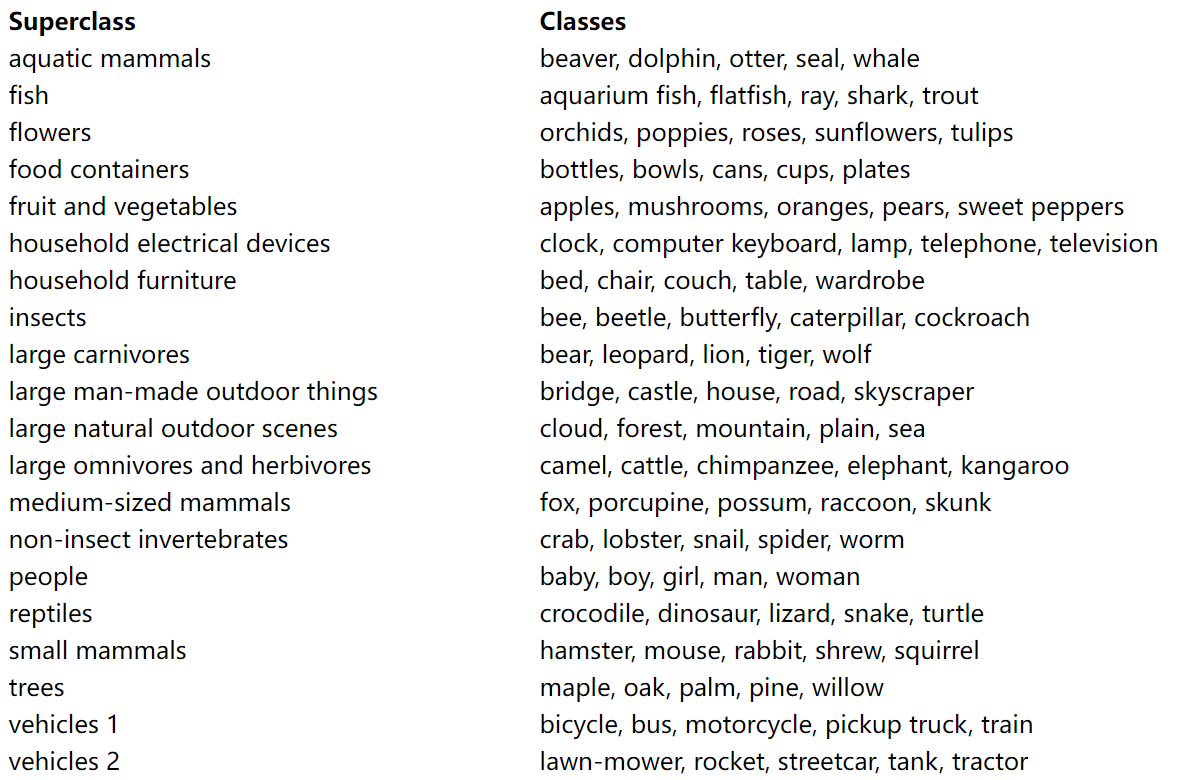
\includegraphics[width=0.90\textwidth]{../img/cifar100-classes.png}
    \caption{CIFAR-100数据集的标签}
\end{figure}

下面展示了CIFAR-100训练集中的9张图像:

\begin{figure}[htbp]
    \centering
    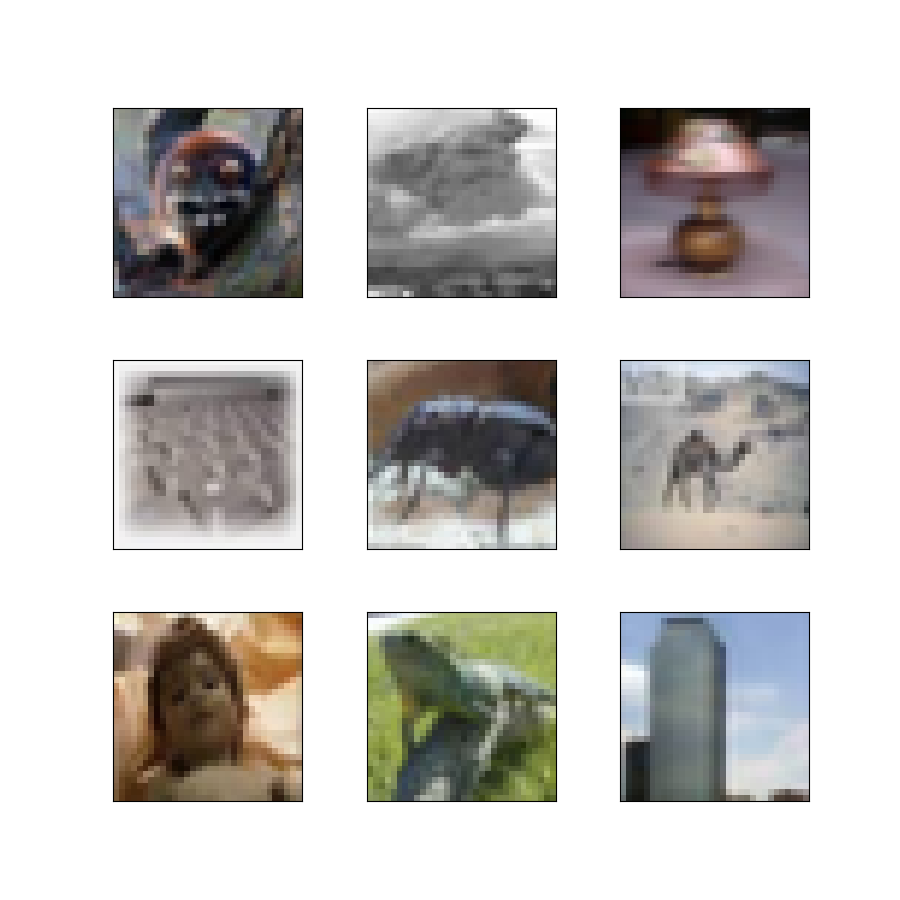
\includegraphics[width=0.30\textwidth]{../img/cifar100.png}
    \caption{CIFAR-100数据集的图像示例}
\end{figure}

\subsection{baseline模型}

\subsubsection{模型基本结构}
残差网络(ResNet)由微软研究院的何恺明、张祥雨、任少卿、孙剑等人在Deep Residual Learning for Image Recognition一文中提出,
在2015年的ILSVRC(ImageNet Large Scale Visual Recognition Challenge)中取得了冠军。
ResNet认为,理论上,可以训练一个相对浅层的网络,然后在这个训练好的相对浅层的网络上堆几层恒等映射层,
即输出等于输入的层,构建出一个更深层的网络。这两个网络得到的结果应该是一模一样的,
因而在训练集上,深层的网络不会比浅层的网络效果差。


ResNet通过加入shortcut connections,变得更加容易被优化。
包含一个shortcut connection的几层网络被称为一个残差块(residual block),如图3所示。


\begin{figure}[htbp]
    \centering
    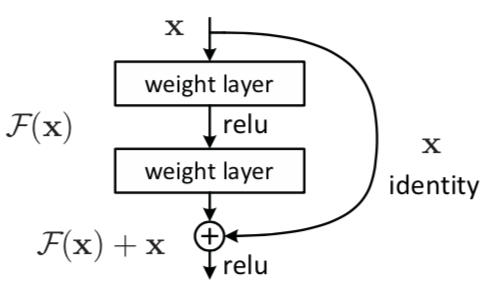
\includegraphics[width=0.40\textwidth]{../img/1-1.png}
    \caption{残差块}
\end{figure}

如图4所示,展示了ResNet的几种结构:

\begin{figure}[htbp]
    \centering
    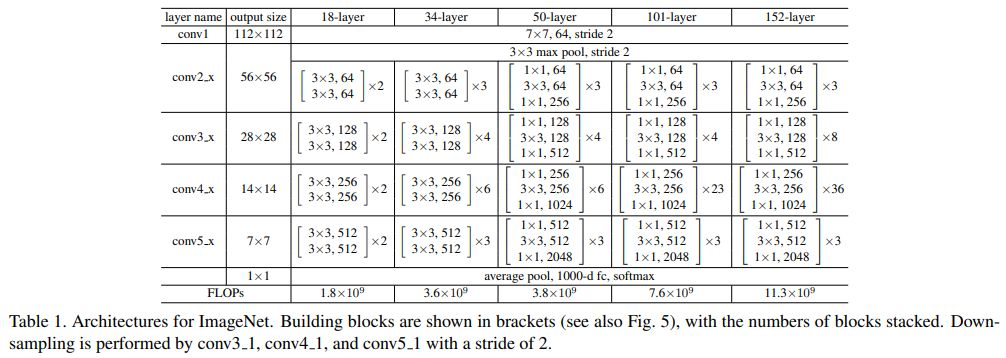
\includegraphics[width=0.90\textwidth]{../img/1-2.jpg}
    \caption{ResNet的几种结构}
\end{figure}

其中,ResNet-18和ResNet-34使用两个$3\times3$的卷积层作为一个块,
而ResNet-50,ResNet-101和ResNet-152将其替换为$1\times1+3\times3+1\times1$的卷积进行计算优化,
这样的块即减少了计算量又能够保持精度,被称为BottleNeck块。

另外,为了使得输入和输出保持相同的维度,若特征图维度不同,
对于卷积层的残差块,需要在$1\times1$卷积后添加批归一化(Batch Normalization)处理,如图5所示。

\begin{figure}[htbp]
    \centering
    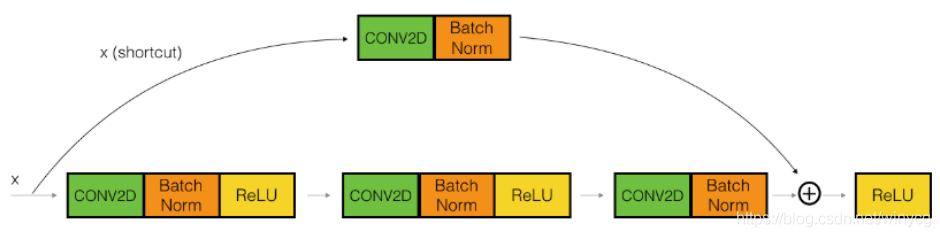
\includegraphics[width=0.90\textwidth]{../img/1-3.png}
    \caption{批归一化}
\end{figure}

考虑到训练的效率,我们使用ResNet-18作为baseline模型。由于CIFAR-100的图像较小,
ResNet-18中的第一层卷积使用$7\times7$卷积核可能过大,难以提取CIFAR-100图像的特征,
我们将其调整为$3\times3$卷积核。此外,模型的其它的baseline如下:
\begin{itemize}
    \item epoch:100
    \item batch size:100
    \item drop out:不使用
    \item 损失函数:交叉熵损失
    \item 正则化:$l_2$正则化,正则化参数$\lambda=10^{-5}$
    \item 优化器:Adam
    \item 动量系数:$\beta_1=0.9, \beta_2=0.999$
    \item 初始学习率:$\alpha=10^{-3}$
    \item 学习率衰减:每个epoch后学习率衰减为上一个epoch的0.98
\end{itemize}

我们得到baseline模型
在测试集上的平均误差为$\textbf{2.455}$,分类精度为$\textbf{0.604}$。
模型的性能曲线如下所示:

\begin{figure}[htbp]
    \centering
    \subfigure[accuracy曲线]{
        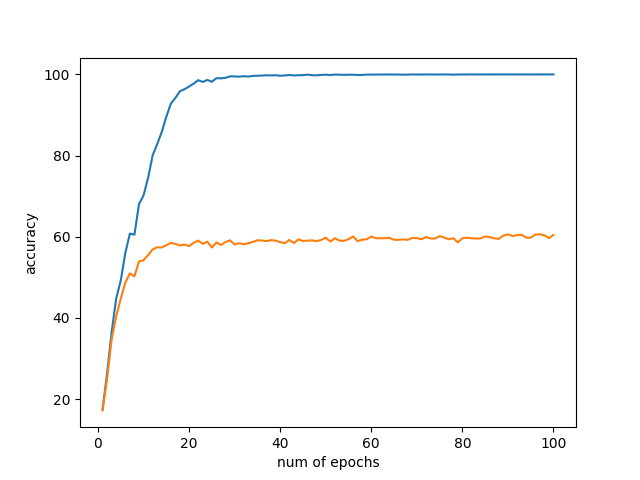
\includegraphics[width=0.40\textwidth]{../img/accuracy1.png}
    }
    \hspace{0.5in}
    \subfigure[loss曲线]{
        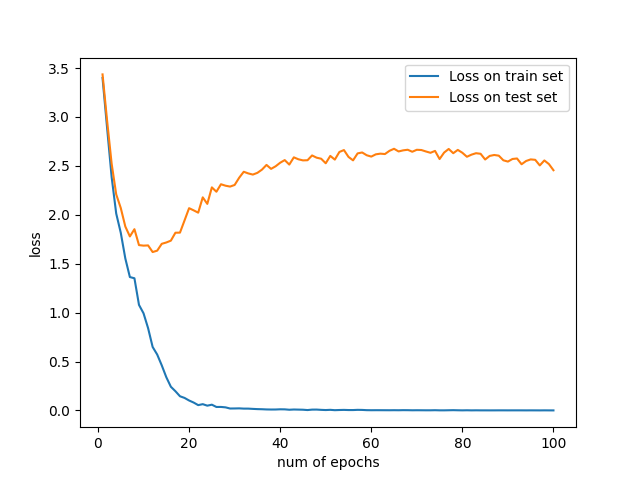
\includegraphics[width=0.40\textwidth]{../img/loss1.png}
    }
    \caption{baseline模型的性能曲线}
\end{figure}

可以发现,模型的精度较低,且模型存在较严重的振荡和过拟合现象。

\subsubsection{模型超参数调整}
为了缓解模型的过拟合现象,我们将baseline模型的超参数进行调整,
以得到较高的精度。调整后模型的超参数如下:
\begin{itemize}
    \item epoch:100
    \item batch size:100
    \item drop out:使用
    \item 损失函数:交叉熵损失
    \item 正则化:$l_2$正则化,正则化参数$\lambda=10^{-3}$
    \item 优化器:SGD
    \item 动量系数:$\beta=0.9$
    \item 初始学习率:$\alpha=10^{-2}$
    \item 学习率衰减:每个epoch后学习率衰减为上一个epoch的0.98
\end{itemize}

经过调整后,我们得到模型
在测试集上的平均误差为$\textbf{1.317}$,分类精度为$\textbf{0.672}$。
模型的性能曲线如下所示:

\begin{figure}[htbp]
    \centering
    \subfigure[accuracy曲线]{
        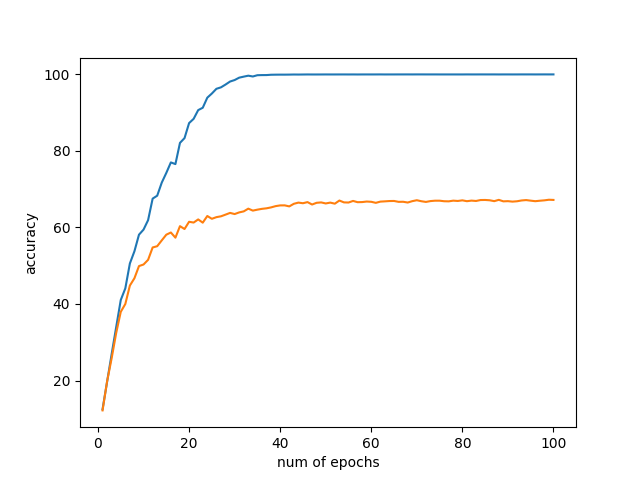
\includegraphics[width=0.40\textwidth]{../img/accuracy2.png}
    }
    \hspace{0.5in}
    \subfigure[loss曲线]{
        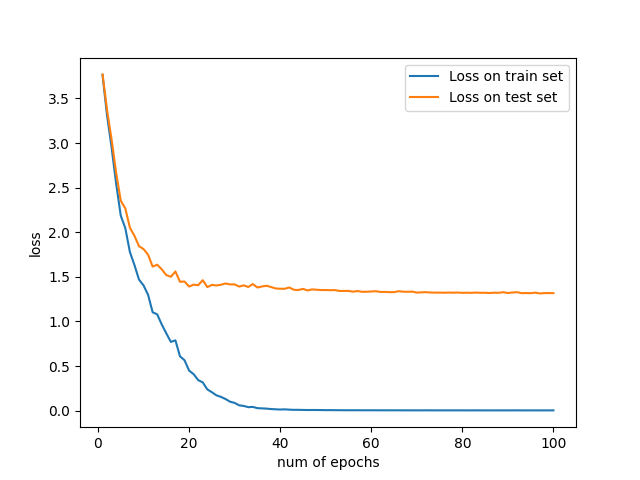
\includegraphics[width=0.40\textwidth]{../img/loss2.png}
    }
    \caption{调整后的性能曲线}
\end{figure}

可以发现,模型的过拟合现象得到了一定程度的改善,精度得到了提高,
且不再出现测试集上loss随训练过程增加的现象。

\subsection{数据增强}

\subsubsection{随机裁剪和水平翻转}
我们可以对模型的数据作一些简单的数据增强。
基于torchvision自带的transforms.RandomCrop和
transforms.RandomHorizontalFlip函数,
我们可以简单地实现对训练集图像进行向四周填充后随机裁剪以及随机翻转的操作。
这两种操作不会对图像的基本信息造成太大影响。

\begin{figure}[htbp]
    \centering
    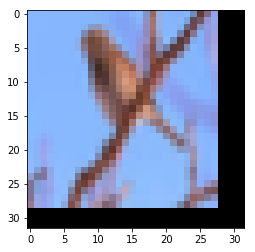
\includegraphics[width=0.20\textwidth]{../img/1-4.png}
    \caption{向四周填充后随机裁剪的效果}
\end{figure}

经过随机裁剪和水平翻转后,我们得到模型
在测试集上的平均误差为$\textbf{1.154}$,
分类Top-1精度为$\textbf{72.2\%}$,
Top-5精度为$\textbf{91.9\%}$。
模型的性能曲线如下所示:

\begin{figure}[htbp]
    \centering
    \subfigure[Top-1 accuracy曲线]{
        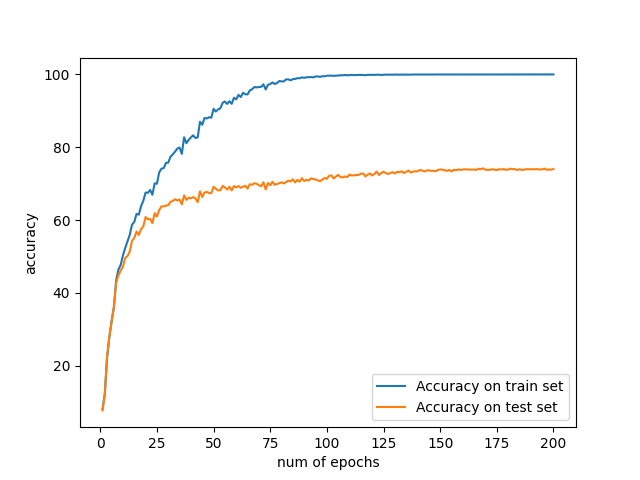
\includegraphics[width=0.40\textwidth]{../img/accuracy3.png}
    }
    \hspace{0.5in}
    \subfigure[Top-5 accuracy曲线]{
        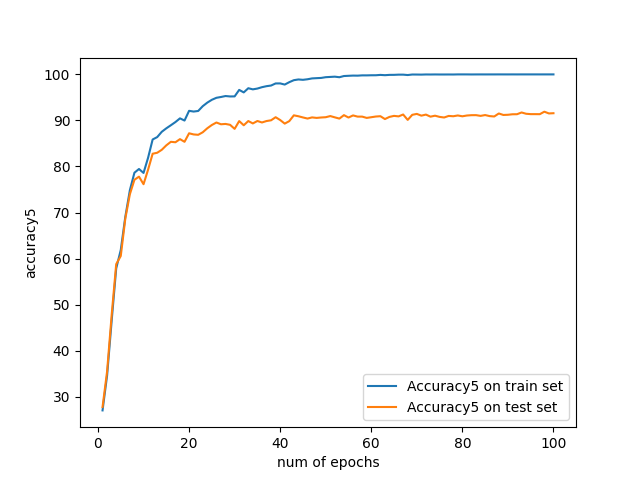
\includegraphics[width=0.40\textwidth]{../img/accuracy3_top5.png}
    }
    \hspace{0.5in}
    \subfigure[loss曲线]{
        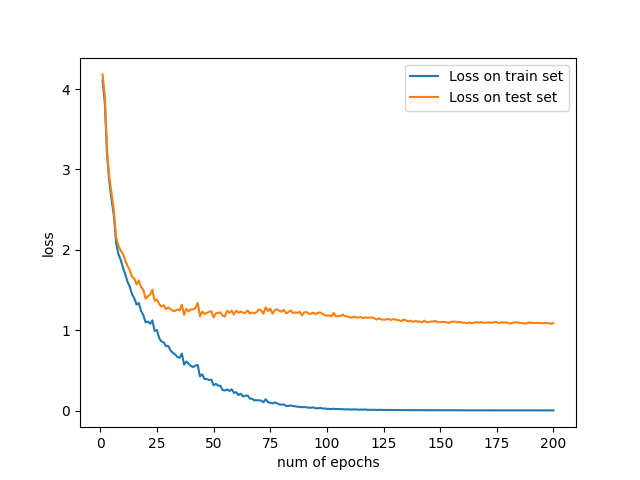
\includegraphics[width=0.40\textwidth]{../img/loss3.png}
    }
    \caption{增强后模型的性能曲线}
\end{figure}

\subsubsection{Cut out}
Cut out的原理是:随机将样本中的部分区域去掉,
然后填充0像素值,分类的结果不变。
如图10所示,展示了三张训练集样本Cut out后的图像。

\begin{figure}[htbp]
    \centering
    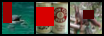
\includegraphics[width=0.40\textwidth]{../img/sample_cutout.png}
    \caption{cutout的效果}
\end{figure}

基于torchtoolbox包自带的Cutout方法,我们在数据增强时增加Cut out操作,
设置对图像进行Cutout的概率为0.5。进行Cut out后,
得到模型在测试集上的平均误差为$\textbf{1.107}$,
分类Top-1精度为$\textbf{72.3\%}$,
Top-5精度为$\textbf{91.6\%}$。
模型的性能曲线如图11所示。

\begin{figure}[htbp]
    \centering
    \subfigure[Top-1 accuracy曲线]{
        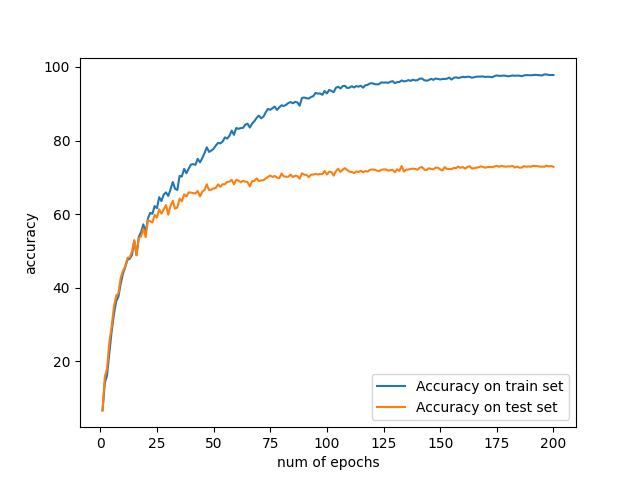
\includegraphics[width=0.40\textwidth]{../img/accuracy4.png}
    }
    \hspace{0.5in}
    \subfigure[Top-5 accuracy曲线]{
        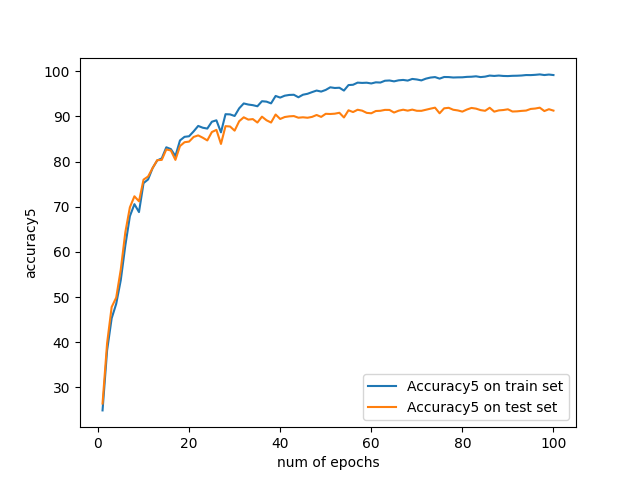
\includegraphics[width=0.40\textwidth]{../img/accuracy4_top5.png}
    }
    \hspace{0.5in}
    \subfigure[loss曲线]{
        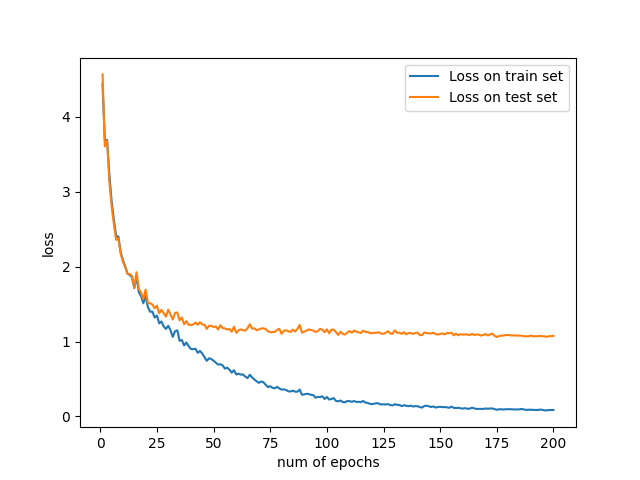
\includegraphics[width=0.40\textwidth]{../img/loss4.png}
    }
    \caption{cutout后模型的性能曲线}
\end{figure}

我们可以可视化五个中间block各一个特征通道的输出,如图12所示:

\begin{figure}[h]
    \centering
    \subfigure[输入层]{
        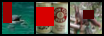
\includegraphics[width=0.20\textwidth]{../img/sample_cutout.png}
    }
    \hspace{0.5in}
    \subfigure[Conv1层输出]{
        
\includegraphics[width=0.20\textwidth]{../img/sample_cutouthidden1.png}
    }
    \hspace{0.5in}
    \subfigure[Conv2层输出]{
        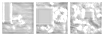
\includegraphics[width=0.20\textwidth]{../img/sample_cutouthidden2.png}
    }
    \hspace{0.5in}
    \subfigure[Conv3层输出]{
        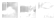
\includegraphics[width=0.20\textwidth]{../img/sample_cutouthidden3.png}
    }
    \hspace{0.5in}
    \subfigure[Conv4层输出]{
        
\includegraphics[width=0.20\textwidth]{../img/sample_cutouthidden4.png}
    }
    \hspace{0.5in}
    \subfigure[Conv5层输出]{
        
\includegraphics[width=0.20\textwidth]{../img/sample_cutouthidden5.png}
    }
    \caption{隐藏层输出可视化}
\end{figure}

\subsubsection{Cut mix}
Cutmix的原理是:将一部分区域去掉,但不是填充随机的固定像素值,
而是随机填充训练集中的其他数据的区域像素值,分类结果按一定的比例分配。

Cutmix可以用公式表示:
$$\begin{aligned}
    \tilde{x} &= \textbf{M} \odot x_A + (\textbf{1}-\textbf{M}) \odot x_B \\
    \tilde{y} &= \lambda y_A + (1-\lambda) y_B
\end{aligned}$$
其中$\lambda\sim Beta(\alpha, \alpha)$,
$\textbf{M}\in\{0,1\}^{W\times H}$表示选择来自哪张图片的掩码,
$\odot$表示逐元素相乘。为此,我们还需要确定一个随机采样得到的bounding box,即
$B=(r_x,r_y,r_w,r_h)$,采样方法为:
$$\begin{aligned}
    & r_x \sim {\rm Unif}(0, W), & \quad r_w=W\sqrt{1-\lambda} \\
    & r_y \sim {\rm Unif}(0, H), & \quad r_h=H\sqrt{1-\lambda}
\end{aligned}$$
这样即可保证裁剪区域的大小为原图像的$1-\lambda$倍。

我们取$\alpha=1$,此时$\lambda\sim{\rm Unif}(0, 1)$。
图13展示了以三张训练集样本作为一个batch,经过cutmix后的图像:

\begin{figure}[htbp]
    \centering
    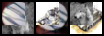
\includegraphics[width=0.40\textwidth]{../img/sample_cutmix.png}
    \caption{cutmix的效果}
\end{figure}

进行cutmix后,我们得到模型
在测试集上的平均误差为$\textbf{1.000}$,
分类Top-1精度为$\textbf{72.9\%}$,
Top-5精度为$\textbf{92.9\%}$。
模型的性能曲线如图14所示。

\begin{figure}[htbp]
    \centering
    \subfigure[Top-1 accuracy曲线]{
        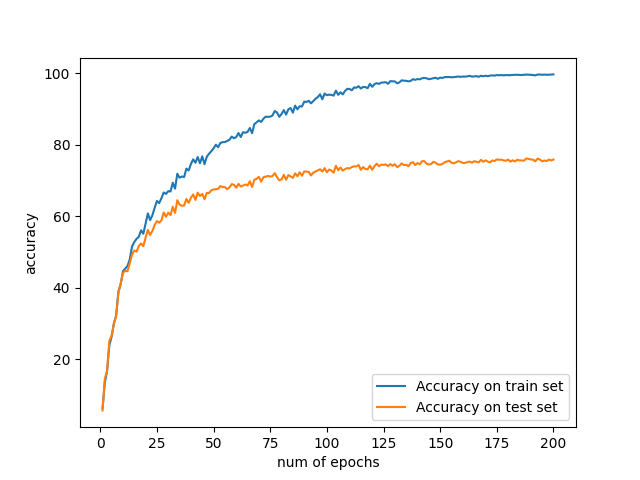
\includegraphics[width=0.40\textwidth]{../img/accuracy5.png}
    }
    \hspace{0.5in}
    \subfigure[Top-5 accuracy曲线]{
        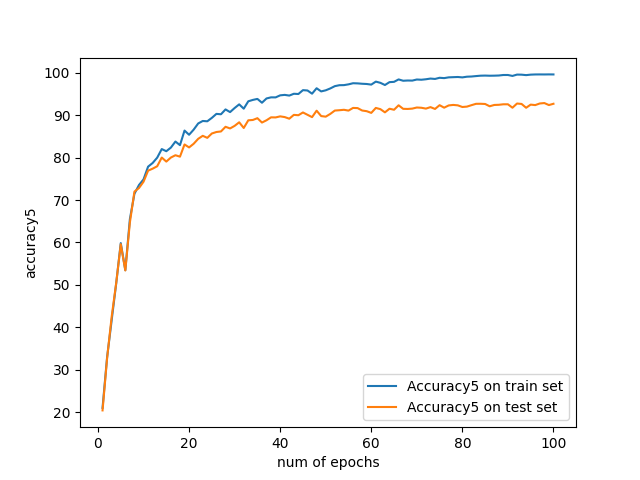
\includegraphics[width=0.40\textwidth]{../img/accuracy5_top5.png}
    }
    \hspace{0.5in}
    \subfigure[loss曲线]{
        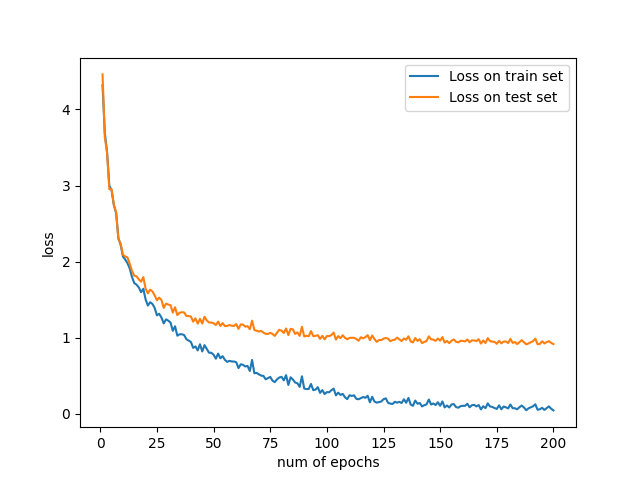
\includegraphics[width=0.40\textwidth]{../img/loss5.png}
    }
    \caption{cutmix后模型的性能曲线}
\end{figure}

可视化五个中间block各一个特征通道的输出,如图15所示。

\begin{figure}[htbp]
    \centering
    \subfigure[输入层]{
        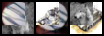
\includegraphics[width=0.20\textwidth]{../img/sample_cutmix.png}
    }
    \hspace{0.5in}
    \subfigure[Conv1层输出]{
        
\includegraphics[width=0.20\textwidth]{../img/sample_cutmixhidden1.png}
    }
    \hspace{0.5in}
    \subfigure[Conv2层输出]{
        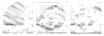
\includegraphics[width=0.20\textwidth]{../img/sample_cutmixhidden2.png}
    }
    \hspace{0.5in}
    \subfigure[Conv3层输出]{
        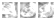
\includegraphics[width=0.20\textwidth]{../img/sample_cutmixhidden3.png}
    }
    \hspace{0.5in}
    \subfigure[Conv4层输出]{
        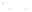
\includegraphics[width=0.20\textwidth]{../img/sample_cutmixhidden4.png}
    }
    \hspace{0.5in}
    \subfigure[Conv5层输出]{
        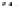
\includegraphics[width=0.20\textwidth]{../img/sample_cutmixhidden5.png}
    }
    \caption{隐藏层输出可视化}
\end{figure}

\newpage
\subsubsection{Mix up}
Mixup的原理是:将两张图按比例进行插值来混合样本。

Mixup可以用公式表示:
$$\begin{aligned}
    \tilde{x} &= \lambda x_A + (1-\lambda) x_B \\
    \tilde{y} &= \lambda y_A + (1-\lambda) y_B
\end{aligned}$$
其中$\lambda\sim Beta(\alpha, \alpha)$

我们取$\alpha=0.2$,如图16所示,
展示了以三张训练集样本作为一个batch,经过Mix up后的图像。

\begin{figure}[h]
    \centering
    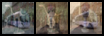
\includegraphics[width=0.40\textwidth]{../img/sample_mixup.png}
    \caption{mixup的效果}
\end{figure}

进行mixup后,我们得到模型
在测试集上的平均误差为$\textbf{1.036}$,
分类Top-1精度为$\textbf{72.5\%}$,
Top-5精度为$\textbf{92.2\%}$。
模型的性能曲线如图17所示。

\begin{figure}[htbp]
    \centering
    \subfigure[Top-1 accuracy曲线]{
        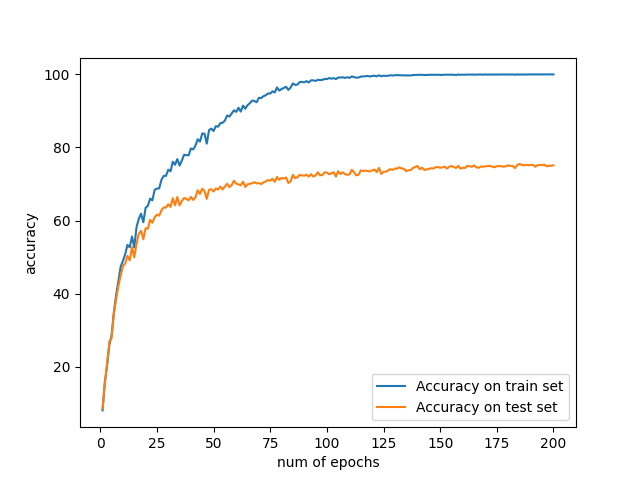
\includegraphics[width=0.40\textwidth]{../img/accuracy6.png}
    }
    \hspace{0.5in}
    \subfigure[Top-5 accuracy曲线]{
        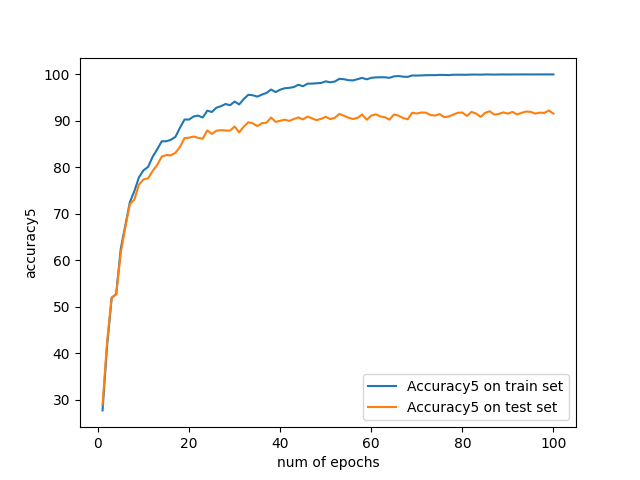
\includegraphics[width=0.40\textwidth]{../img/accuracy6_top5.png}
    }
    \hspace{0.5in}
    \subfigure[loss曲线]{
        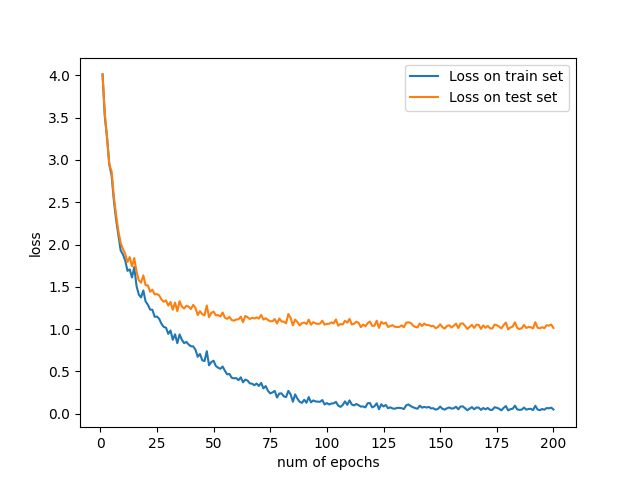
\includegraphics[width=0.40\textwidth]{../img/loss6.png}
    }
    \caption{mixup后模型的性能曲线}
\end{figure}

可视化五个中间block各一个特征通道的输出,如图18所示。

\begin{figure}[h]
    \centering
    \subfigure[输入层]{
        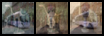
\includegraphics[width=0.20\textwidth]{../img/sample_mixup.png}
    }
    \hspace{0.5in}
    \subfigure[Conv1层输出]{
        
\includegraphics[width=0.20\textwidth]{../img/sample_mixuphidden1.png}
    }
    \hspace{0.5in}
    \subfigure[Conv2层输出]{
        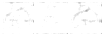
\includegraphics[width=0.20\textwidth]{../img/sample_mixuphidden2.png}
    }
    \hspace{0.5in}
    \subfigure[Conv3层输出]{
        
\includegraphics[width=0.20\textwidth]{../img/sample_mixuphidden3.png}
    }
    \hspace{0.5in}
    \subfigure[Conv4层输出]{
        
\includegraphics[width=0.20\textwidth]{../img/sample_mixuphidden4.png}
    }
    \hspace{0.5in}
    \subfigure[Conv5层输出]{
        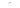
\includegraphics[width=0.20\textwidth]{../img/sample_mixuphidden5.png}
    }
    \caption{隐藏层输出可视化}
\end{figure}

\subsection{小结}
我们总共得出下面四个模型:
\begin{itemize}
    \item baseline模型(ResNet-18,经过超参数调整)
    \item baseline模型 + cutout
    \item baseline模型 + cutmix
    \item baseline模型 + mixup
\end{itemize}

四个模型在测试集上的loss和accurary如下表所示:

\begin{table}[!ht]
    \begin{center}
        \begin{tabular}{cccc}
            \hline
            模型  & 测试集误差 & 测试集Top-1精度 & 测试集Top-5精度 \\ \hline
            baseline & 1.154 & 72.2\% & 91.9\% \\ \hline
            baseline + cutout & 1.107 & 72.3\% & 91.6\% \\ \hline
            baseline + cutmix & 1.000 & 72.9\% & 92.9\% \\ \hline
            baseline + mixup & 1.036 & 72.5\% & 92.2\% \\ \hline
            \end{tabular}
        \caption{不同数据增强方式对模型性能的影响}
    \end{center}
\end{table}

我们发现,在baseline模型上,增加cutmix方法对数据进行增强,
相对于cutout和mixup两种方法达到的测试集上的误差最小,精度最高。
可以总结出cutmix的以下几个优点:
\begin{itemize}
    \item 在训练过程中不会出现非信息像素,从而能够提高训练效率;
    \item 保留了cutout方法regional dropout的优势,能够关注目标的non-discriminative parts;
    \item 通过要求模型从局部视图识别对象,对cut区域中添加其他样本的信息,能够进一步增强模型的定位能力;
    \item 相较于mixup方法,不会有图像混合后不自然的情形,能够提升模型分类的表现;
    \item 训练和推理的代价保持不变。
\end{itemize}

\newpage

\section{在VOC数据集上训练Faster R-CNN和YOLO V3}

\subsection{数据集介绍与划分}

\subsubsection{数据集总体概况}
PASCAL对于目标检测或分割类型来说属于先驱者的地位。
对于现在的研究者来说比较重要的两个年份的数据集是 $\textbf{PASCAL VOC 2007}$ 
与 $\textbf{PASCAL VOC 2012}$,
这两个数据集频频在现在的一些检测或分割类的论文当中出现。

由于从2007年之后,PASCAL VOC的测试集均不再公布,
因此我们选择PASCAL VOC 2007作为我们的数据集。
下面展示了PASCAL VOC 2007数据集的20个类别及其层级结构:
\begin{figure}[htbp]
    \centering
    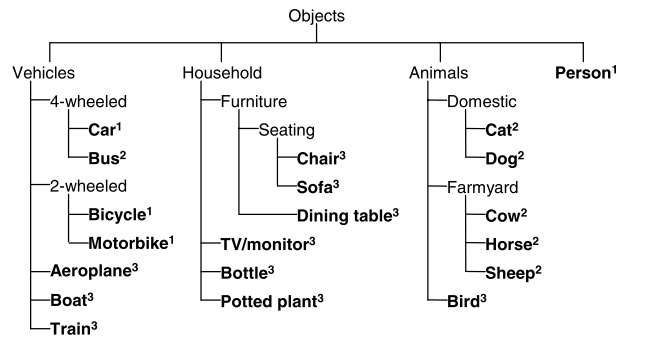
\includegraphics[width=0.90\textwidth]{../img/VOC2007-classes.png}
    \caption{VOC 2007数据集的标签}
\end{figure}

其中:
\begin{itemize}
    \item 分为4个大类,20个小类。预测时主要输出的小类。
    \item 数据集主要关注分类和检测,也就是分类和检测用到的数据集相对规模较大。关于其他任务比如分割,动作识别等,其数据集一般是分类和检测数据集的子集。
\end{itemize}

如图20所示,展示了PASCAL VOC 2007数据集总体的统计情况。
\begin{figure}[htbp]
    \centering
    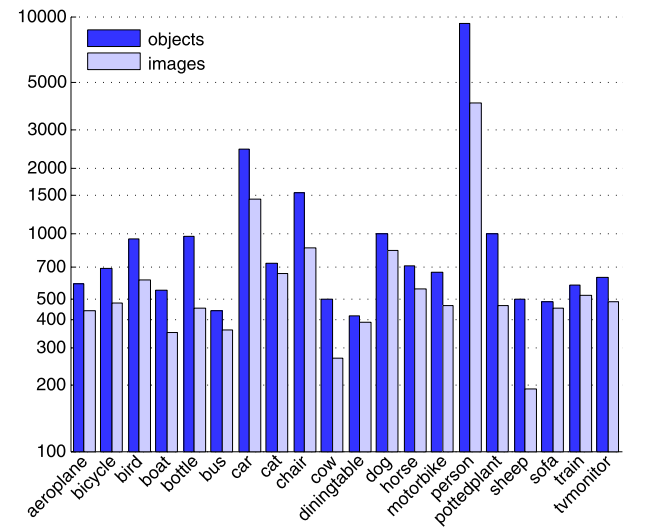
\includegraphics[width=0.60\textwidth]{../img/VOC2007-histogram.png}
    \caption{VOC 2007数据集的统计情况}
\end{figure}

\subsubsection{数据集划分}
PASCAL VOC 2007数据集分为两部分:训练和验证集trainval,测试集test,
两部分各占数据总量的约 50\%。
其中trainval又分为训练集和测试集,二者分别各占trainval的50\%。
每张图片中有可能包含不只一个目标object。

如图21所示,展示了数据集在训练集,验证集,测试集上的划分情况。
\begin{figure}[htbp]
    \centering
    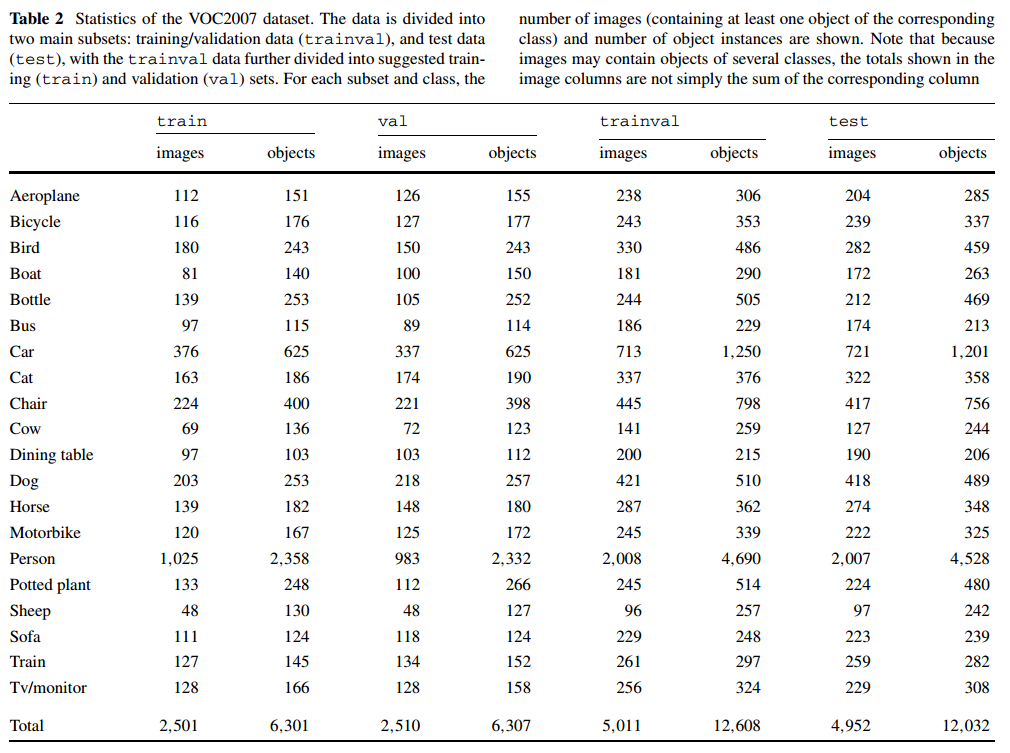
\includegraphics[width=1.00\textwidth]{../img/VOC2007-stats.png}
    \caption{VOC 2007数据集的具体划分情况}
\end{figure}

\subsubsection{数据集可视化}
\url{http://host.robots.ox.ac.uk/pascal/VOC/voc2007/examples/index.html}

网站中展示了VOC-2007中至少包含每个类一个目标的8张图像及其目标的ground truth位置。
下面展示一部分:
\begin{figure}[h]
    \centering
    \subfigure[Aeroplanes]{
        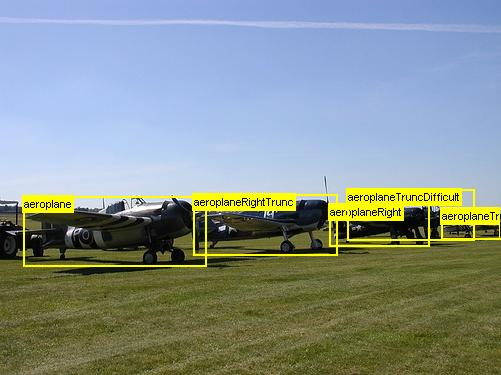
\includegraphics[width=0.40\textwidth]{../img/VOC2007-sample1.jpg}
    }
    \hspace{0.5in}
    \subfigure[Bicycles]{
        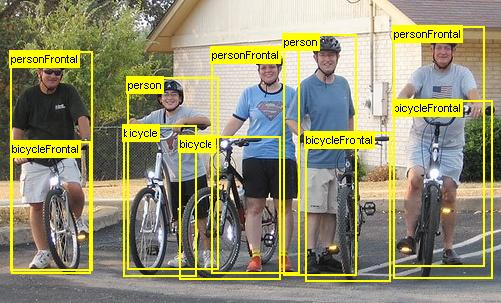
\includegraphics[width=0.40\textwidth]{../img/VOC2007-sample2.jpg}
    }
    \hspace{0.5in}
    \subfigure[Birds]{
        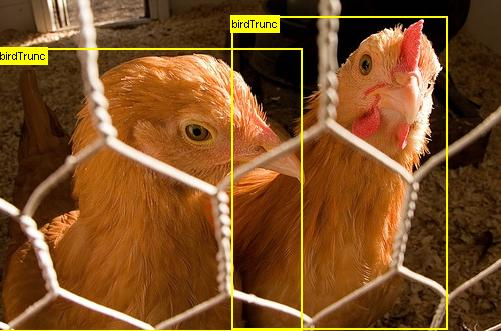
\includegraphics[width=0.40\textwidth]{../img/VOC2007-sample3.jpg}
    }
    \hspace{0.5in}
    \subfigure[Boats]{
        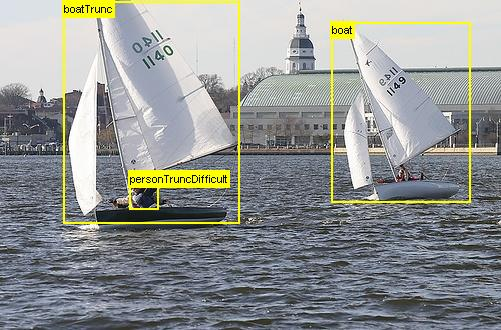
\includegraphics[width=0.40\textwidth]{../img/VOC2007-sample4.jpg}
    }
    \hspace{0.5in}
    \subfigure[Bottles]{
        \includegraphics[width=0.40\textwidth]{../img/VOC2007-sample5.jpg}
    }
    \hspace{0.5in}
    \subfigure[Buses]{
        \includegraphics[width=0.40\textwidth]{../img/VOC2007-sample6.jpg}
    }
    \caption{VOC 2007数据集示例}
\end{figure}

\subsubsection{读取VOC数据集}
使用torchvision.datasets包中的VOCDetection下载数据集,在VOC2007文件夹中,得到下面几个部分:
\begin{itemize}
    \item Annotations:包含了记录图像和标签信息的xml文件
    \item ImageSets:主要包含划分的训练集和测试集中图片的名称
    \item JPEGImages:包含数据集的原始图片
    \item SegmentationClass:按类别分割的ground truth位置
    \item SegmentationObject:按对象分割的ground truth位置
\end{itemize}

我们读取了四张训练集的图像并对其目标的ground truth进行了标注:
\begin{figure}[h]
    \centering
    \subfigure[图片1]{
        \includegraphics[width=0.40\textwidth]{../img/image_0.png}
    }
    \hspace{0.5in}
    \subfigure[图片2]{
        \includegraphics[width=0.40\textwidth]{../img/image_1.png}
    }
    \hspace{0.5in}
    \subfigure[图片3]{
        \includegraphics[width=0.40\textwidth]{../img/image_2.png}
    }
    \hspace{0.5in}
    \subfigure[图片4]{
        \includegraphics[width=0.40\textwidth]{../img/image_3.png}
    }
    \caption{VOC 2007训练集图像ground truth标注示例}
\end{figure}

\subsection{Faster R-CNN模型}
\subsubsection{基本结构}
经过R-CNN和Fast R-CNN的积淀,Ross B. Girshick在2016年提出了新的Faster R-CNN,
在结构上,Faster R-CNN已经将特征抽取(feature extraction),proposal提取,
bounding box regression(rect refine),classification都整合在了一个网络中,
使得综合性能有较大提高,在检测速度方面尤为明显。

整个Faster R-CNN分为4大部分:
共享卷积网络,候选检测框生成网络RPN(Region Proposal Networks),
感兴趣区域池化RoI(Region of Interest)Pooling和分类器。
如图24所示。

\begin{figure}[htbp]
    \centering
    \includegraphics[width=0.60\textwidth]{../img/fasterR-CNN.jpg}
    \caption{Faster R-CNN基本结构}
\end{figure}

其中:
\begin{itemize}
    \item 共享卷积网络(Conv layers):提取image的feature maps。
    该feature maps被共享用于后续RPN层和全连接层。
    \item 候选检测框生成网络(RPN):RPN网络用于生成region proposals。该层通过softmax判断anchors
    属于positive或者negative,再利用bounding box regression
    修正anchors获得精确的proposals。
    \item 感兴趣区域池化(RoI Pooling):该层收集输入的feature maps和proposals,
    综合这些信息后提取proposal feature maps,送入后续全连接层判定目标类别。
    \item 分类器(classifier):利用proposal feature maps计算proposal的类别,
    同时再次bounding box regression获得检测框最终的精确位置。
\end{itemize}

\subsubsection{特征金字塔网络(FPN)}
注意到,上面我们提到的最基本的Faster R-CNN有一个明显的缺陷,即小物体本身具有的像素信息较少,
在下采样的过程中极易被丢失。
FPN(Feature Pyramid Network)算法可以同时利用低层特征高分辨率和高层特征的高语义信息,
通过融合这些不同层的特征达到很好的预测效果。

\begin{figure}[h]
    \centering
    \includegraphics[width=0.50\textwidth]{../img/FPN.png}
    \caption{FPN基本结构}
\end{figure}

如图25所示,左侧模型叫bottom-up,右侧模型叫top-down,
横向的箭头叫横向连接lateral connections。
特征金字塔网络相当于先进行传统的
自上而下的特征卷积,
然后FPN试图融合左侧特征图的相邻的特征图。
具体做法是两个特征层的较高层特征2倍上采样
(一般采用内插值方法,
即在原有图像像素的基础上在像素点之间采用合适的插值算法插入新的元素),
较低层特征通过1×1卷积改变一下低层特征的通道数,
然后简单地把将上采样和1×1卷积后的结果对应元素相加。

\subsubsection{候选检测框生成网络(RPN)}
下面对RPN部分进行详细分析,网络的详细结构如图26所示。

\begin{figure}[htbp]
    \centering
    \includegraphics[width=1.00\textwidth]{../img/fasterR-CNN_details.png}
    \caption{Faster R-CNN结构}
\end{figure}

\begin{itemize}
    \item 特征图上每个位置都对应生成五种面积($32^2,64^2,128^2,256^2,512^2$)
    以及三种比例(1:1,1:2,2:1)的anchor,每个anchor有对应的前景概率及左上、右下角坐标。
    \item 对于一张1000*60*3的图像,大约有20k个anchor,忽略跨越边界的anchor以后,剩下大约6k个anchor。
    对于RPN生成的候选框之间存在大量的重叠,基于候选框的cls得分,采用非极大值抑制,Iou设为0.7,这样每张图片只剩2k个候选框。
    \item 对于IoU$\ge$0.7或和某个ground truth重叠最大的anchor设置为正样本,Iou$\le$0.3作为负样本,其余样本舍去。 
\end{itemize}

计算RPN损失:
$$L(\{p_i\},\{t_i\})=\frac{1}{N_{cls}}\sum_iL_{cls}(p_i,p_i^*)+\lambda\frac{1}{N_{reg}}\sum_ip_i^*L_{reg}(t_i,t_i^*) $$

$$L_{cls}=-[p_i^* \log (p_i)+(1-p_i^*) \log (1-p_i)]$$

$$L_{reg}=\sum_i{\rm smooth}_{L_1}(t_i-t_i^*)$$


\begin{equation}
{\rm smooth}_{L_1}(x)=
\begin{cases}
0.5x^2,& |x|<1\\
|x|-0.5,& otherwise
\end{cases}
\end{equation}

\begin{itemize}
    \item $p_i$表示第i个anchor预测为真实标签的概率
    \item $p_i^*$当正样本是为1,负样本时为0
    \item $t_i$表示第i个anchor预测的边界框回归参数
    \item $t_i^*$表示第i个anchor对应的GT Box
\end{itemize}

\subsubsection{模型训练}

我们采用RPN Loss+Fast R-CNN Loss联合训练方法:
\begin{itemize}
    \item 利用ImageNet预训练分类模型初始化前置卷积网络层参数,并单独训练RPN网络参数
    \item 固定RPN网络的卷积层和全连接层参数,再利用预训练分类模型初始化前置卷积网络参数,
    并利用RPN网络生成的目标建议框去训练Fast R-CNN网络参数。
    \item 固定利用Fast R-CNN训练好的前置卷积网络层参数,微调RPN网络卷积层及全连接层参数。
    \item 固定前置卷积网络层参数,微调Fast R-CNN全连接层参数。最后RPN网络和Fast R-CNN构成统一网络。
\end{itemize}

~\\

训练细节:
\begin{itemize}
    \item epoch=15,由于使用了预训练分类模型,收敛较快
    \item batch size=4,过大会导致报错
    \item 采用学习率下降策略,每3个epochs下降一次
    \item 优化器使用SGD,loss function上文中已经介绍
\end{itemize}


\subsubsection{模型评价}

下面展示了训练过程中的mAP图像,以及学习率和loss图像:
\begin{figure}[H]
    \centering
    \subfigure[mAP]{
        \includegraphics[width=0.3\textwidth]{../img/mAP.png}
    }
    \hspace{0.5in}
    \subfigure[loss]{
        \includegraphics[width=0.3\textwidth]{../img/loss.png}
    }
    \hspace{0.5in}
    \subfigure[loss]{
        \includegraphics[width=0.3\textwidth]{../img/lr.png}
    }
    \caption{训练过程的mAP,loss和学习率}
\end{figure}

我们得到最终模型的性能指标如下:

\begin{table}[H]
    \begin{center}
        \begin{tabular}{ccc}
            \hline
            mAP@IoU=0.5  & mAP@IoU=0.5:0.95 & mAR@IoU=0.5:0.95 \\ \hline
            0.828 & 0.526 & 0.640 \\ \hline
            \end{tabular}
        \caption{模型性能指标}
    \end{center}
\end{table}

\subsubsection{模型可视化}

我们在四张测试图像上可视化Faster R-CNN第一阶段的proposal box,并
在网上寻找了三张不在VOC数据集中的图片,并使用训练好的模型进行标注:

\begin{figure}[htbp]
    \centering
    \subfigure[9950]{
        \includegraphics[width=0.3\textwidth]{../img/test_result7.jpg}
    }
    \subfigure[9954]{
        \includegraphics[width=0.3\textwidth]{../img/test_result6.jpg}
    }
    \hspace{0.5in}
    \subfigure[9955]{
        \includegraphics[width=0.3\textwidth]{../img/test_result5.jpg}
    }
    \hspace{0.5in}
    \subfigure[9958]{
        \includegraphics[width=0.3\textwidth]{../img/test_result4.jpg}
    }
    \caption{proposal box}
\end{figure}

\begin{figure}[htbp]
    \centering
    \subfigure[图片1]{
        \includegraphics[width=0.3\textwidth]{../img/test_result1.jpg}
    }
    \hspace{0.5in}
    \subfigure[图片2]{
        \includegraphics[width=0.3\textwidth]{../img/test_result2.jpg}
    }
    \hspace{0.5in}
    \subfigure[图片3]{
        \includegraphics[width=0.3\textwidth]{../img/test_result3.jpg}
    }
    \caption{网上搜索的图像标注结果}
\end{figure}

\newpage
\subsection{YOLO V3模型}

\subsubsection{YOLO V3基本结构}
相较于两阶段的检测模型Faster R-CNN,
Joseph Redmon和Ali Farhadi等人的YOLO提供了另一种更为直接的思路: 
直接在输出层回归bounding box的位置和bounding box所属的类别
(整张图作为网络的输入,把目标的问题转化成一个回归问题)。

YOLO V3模型(基于COCO数据集,检测物体分为80类)的基本结构如下所示:

\begin{figure}[htbp]
    \centering
    \includegraphics[width=1.0\textwidth]{../img/YOLOv3.png}
    \caption{YOLO V3基本结构}
\end{figure}

其中:
\begin{itemize}
    \item 输入:把大小为$416\times416$的输入图像划分成$S×S$大小的grid cell,
    然后对每个cell都预测$B=3$个bounding boxes,
    每个bounding box都包含5个预测值:$(x,y,w,h,{\rm confidence})$。
    \begin{itemize}
        \item $(x,y)$:bounding box的中心坐标
        \item $(w,h)$:相对于cell大小进行归一化后bounding box的宽和高,注意这里使用了sigmoid函数
        \item ${\rm confidence}$:代表了所预测的box中含有目标的置信度和这个box预测有多准两重信息
    \end{itemize}
    \item backbone网络:DarkNet-53,
    其中包括若干个卷积层和批归一化层,但不包括池化层(用一定步长的卷积代替)和全连接层,
    使用Leaky-ReLU作为激活函数。
    \begin{itemize}
        \item DBL:DarkNet的基本块,包括卷积、批归一化和Leaky ReLU
        \item resn:使用了n个残差连接的块,其中res\_unit表示将残差连接
        \item concat:张量拼接,将DarkNet中间层和后面的某一层的上采样进行拼接。
    \end{itemize}
    \item 支路预测:为了加强算法对小目标检测的精确度,
    YOLO V3中采用类似FPN的上采样和融合做法,在多个尺度($13\times13,26\times26,52\times52$)的特征图上做检测,
    这相当于分别对原图像进行了$32,16,8$倍的降采样。
    \item 输出:针对80类,每个cell对应的输出应为$3\times(80+4+1)=255$,因此有上图所示的三种输出
\end{itemize}

\begin{figure}[htbp]
    \centering
    \includegraphics[width=0.40\textwidth]{../img/darknet53.png}
    \caption{DarkNet-53}
\end{figure}

\subsubsection{YOLO V3的anchor box}
从YOLO V2开始,引入了Faster R-CNN中人工设计的anchor box。
这存在一个弊端,就是并不能保证它们一定能很好的适合数据集,
YOLO V2中提到了这个问题,并使用K-means聚类来代替人工设计,
通过对训练集的bounding box进行聚类,自动生成一组更加适合数据集的anchor,
可以使网络的检测效果更好。
如果anchor的尺寸和目标的尺寸差异较大,
则会影响模型的检测效果。

在YOLO V3中,32倍降采样的感受野最大,适合检测大的目标,
所以在输入为416×416时,每个cell的三个anchor box为(116, 90), (156, 198), (373, 326);
16倍适合一般大小的物体,anchor box为(30, 61), (62, 45), (59, 119);
8倍的感受野最小,适合检测小目标,anchor box为(10, 13), (16, 30), (33, 23)。
所以当输入为$416\times416$时,
实际总共有$(52\times52+26\times26+13\times13)\times3=10647$
个proposal box。

引入anchor box的时候遇到的另一个问题是:模型不稳定,尤其是在训练刚开始的时候。
因此,相较于Faster R-CNN的无约束预测
$$\begin{aligned}
    x &= (t_x \times w_a) + x_a \\
    y &= (t_y \times h_a) + y_a
\end{aligned}$$

YOLO V3预测的则是边界框中心点相对于对应cell左上角位置的相对偏移值:
$$\begin{aligned}
    b_x &= \sigma(t_x) + c_x \\
    b_y &= \sigma(t_y) + c_y \\
    b_w &= p_w \exp(t_w) \\
    b_h &= p_h \exp(t_h)
\end{aligned}$$

其中$p_w,p_h$指anchor box的宽和高,
$c_x,c_y$指cell左上角相对于image左上角的距离,
$t_x,t_y,t_w,t_h$为每个bounding box预测的值。

\subsubsection{YOLO V3损失函数}
为了计算损失函数,我们首先需要选择正负样本。
其中,正样本表示负责预测目标的样本,负样本表示负责预测背景的样本。
正负样本是按照以下规则决定的:
如果一个预测框与所有的Ground Truth的最大${\rm IoU}<{\rm ignore\ thresh}$时,那这个预测框就是负样本。
如果Ground Truth的中心点落在一个区域中,
该区域就负责检测该物体。
将与该物体有最大IoU的预测框作为正样本
(注意这里没有用到ignore thresh,即使该最大
${\rm IoU}<{\rm ignore\ thresh}$也不会影响该预测框为正样本)

在YOLOv3中,Loss分为三个部分:
\begin{itemize}
    \item 定位误差,也即计算bounding box带来的loss
    \item 置信度误差,bounding box中是否含有物体的概率,也就是obj带来的loss
    \item 分类误差,也就是class带来的loss
\end{itemize}

用公式表示即:
$$\begin{aligned}
    loss &= l_{\rm box} + l_{\rm obj} + l_{\rm cls} \\
    l_{\rm box} &= \lambda_{\rm coord}\sum_{i=0}^{S^2}
    \sum_{j=0}^{B}1_{i,j}^{obj}(2-w_ih_i)
    [(x_i-\hat{x_i})^2+(y_i-\hat{y_i})^2+(w_i-\hat{w_i})^2+(h_i-\hat{h_i})^2] \\
    l_{\rm cls} &= \lambda_{\rm class}\sum_{i=0}^{S^2}
    \sum_{j=0}^{B}1_{i,j}^{obj}\sum_{c\in classes}p_i(c)\log(\hat{p}_i(c)) \\
    l_{\rm obj}&= \lambda_{\rm obj}\sum_{i=0}^{S^2}
    \sum_{j=0}^{B}1_{i,j}^{obj}(c_i-\hat{c}_i)^2+
    \lambda_{\rm noobj}\sum_{i=0}^{S^2}
    \sum_{j=0}^{B}1_{i,j}^{noobj}(c_i-\hat{c}_i)^2
\end{aligned}$$

其中:
\begin{itemize}
    \item $S$:gird cell的大小,分为三种(见2.3.2)
    \item $B$:bounding box的个数
    \item $1_{i,j}^{obj}$:若在$(i,j)$的box有目标,则为1,否则为0
    \item $1_{i,j}^{noobj}$:若在$(i,j)$的box没有目标,则为1,否则为0
\end{itemize}

需要注意的是,定位误差中,我们使用了GIoU代替IoU,其计算方法为
$$GIoU=IoU-\dfrac{|A_c-U|}{|A_c|}$$

其中:
\begin{itemize}
    \item $A_c$:两个框构成的最小闭包面积,也即同时包含了预测框和真实框的最小框的面积
    \item $U$:两个框的并集面积
\end{itemize}

\subsubsection{YOLO V3 SPP}

SPP全称为Spatial Pyramid Pooling(空间金字塔池化结构),
由何恺明提出,有效避免了对图像区域剪裁、缩放操作导致的图像失真等问题;
同时解决了卷积神经网络对图像重复特征提取的问题,大大提高了产生候选框的速度,且节省了计算成本。

\begin{figure}[h]
    \centering
    \includegraphics[width=0.9\textwidth]{../img/YOLOv3-SPP.png}
    \caption{YOLO V3-SPP基本结构}
\end{figure}

在YOLOv3-SPP中,SPP module由四个并行的分支构成,
分别是kernel size为 $5\times5, 9\times9, 13\times13$
的最大池化和一个跳跃连接。
特征图经过局部特征与全局特征相融合后,
丰富了特征图的表达能力,
有利于待检测图像中目标大小差异较大的情况,
尤其是对于YOLOv3这种复杂的多目标检测,所以对检测的精度上有了很大的提升。

\begin{figure}[h]
    \centering
    \includegraphics[width=0.5\textwidth]{../img/SPP.png}
    \caption{SPP}
\end{figure}

\subsubsection{模型训练}

我们在官方提供的预训练模型下训练,经过超参数调整,我们设置的模型超参数如下:

\begin{itemize}
    \item epoch:30
    \item 优化器:SGD+momentum,设置动量系数为0.937
    \item 损失函数:前面已给出,包含三项(定位误差、置信度误差和分类误差)
    \item 损失函数权重:
    \begin{itemize}
        \item $\lambda_{\rm coord}=3.54$
        \item $\lambda_{\rm class}=37.4$
        \item $\lambda_{\rm obj}=64.3$
    \end{itemize}
    \item 正则化:$l_2$,设置正则化参数为0.0005
    \item 学习率:初始学习率为1e-3,在训练过程中以余弦方式衰减至1e-5
    \item 样本选取IoU阈值:0.2
\end{itemize}

同时,我们使用了HSV转换的数据增强方法,
对训练图像的色相、饱和度和灰度作随机抖动。

\subsubsection{模型评价}

下面给出Tensorboard中显示的学习率以及各项损失函数的曲线:

\begin{figure}[h]
    \centering
    \subfigure[学习率]{
        \includegraphics[width=0.40\textwidth]{../img/yolo_lr.png}
    }
    \hspace{0.5in}
    \subfigure[总损失函数]{
        \includegraphics[width=0.40\textwidth]{../img/yolo_loss.jpg}
    }
    \hspace{0.5in}
    \subfigure[定位损失]{
        \includegraphics[width=0.25\textwidth]{../img/yolo_giou_loss.jpg}
    }
    \hspace{0.5in}
    \subfigure[置信度损失]{
        \includegraphics[width=0.25\textwidth]{../img/yolo_obj_loss.jpg}
    }
    \hspace{0.5in}
    \subfigure[分类损失]{
        \includegraphics[width=0.25\textwidth]{../img/yolo_cls_loss.jpg}
    }
    \caption{学习率和损失函数曲线}
\end{figure}

我们得到最终模型的性能指标如下:

\begin{table}[!ht]
    \begin{center}
        \begin{tabular}{ccc}
            \hline
            mAP@IoU=0.5  & mAP@IoU=0.5:0.95 & mAR@IoU=0.5:0.95 \\ \hline
            0.806 & 0.565 & 0.682 \\ \hline
            \end{tabular}
        \caption{模型性能指标}
    \end{center}
\end{table}

对应训练过程中的mAP和mAR曲线如图32所示。

\begin{figure}[h]
    \centering
    \subfigure[mAP@IoU=0.5]{
        \includegraphics[width=0.40\textwidth]{../img/yolo_mAP0.5_0.95.png}
    }
    \hspace{0.5in}
    \subfigure[mAP@IoU=0.5:0.95]{
        \includegraphics[width=0.40\textwidth]{../img/yolo_mAP_0.5.png}
    }
    \hspace{0.5in}
    \subfigure[mAR@IoU=0.5:0.95]{
        \includegraphics[width=0.40\textwidth]{../img/yolo_mAR_0.5_0.95.png}
    }
    \caption{训练过程曲线}
\end{figure}


\subsubsection{模型可视化}

我们使用可视化Faster R-CNN中三张不在VOC数据集中的图片,并使用训练好的模型进行标注。
\begin{figure}[!ht]
    \centering
    \subfigure[图片1]{
        \includegraphics[width=0.3\textwidth]{../img/test1_result2.jpg}
    }
    \subfigure[图片2]{
        \includegraphics[width=0.3\textwidth]{../img/test2_result2.jpg}
    }
    \hspace{0.5in}
    \subfigure[图片3]{
        \includegraphics[width=0.3\textwidth]{../img/test3_result2.jpg}
    }
    \caption{网上搜索的图像标注结果}
\end{figure}

值得注意的是,图片3中,有一个人未被检测出,
这是Faster R-CNN不曾表现出的误差。

\subsection{小结}
在本节中,我们分别使用目标检测模型:两阶段的$\textbf{Faster R-CNN}$
和单阶段的$\textbf{YOLOv3-SPP}$在VOC2007数据集上训练。

Faster R-CNN通过将region proposal整合到CNN模型来提高速度:
构建由RPN和具有共享卷积特征层的Fast R-CNN组成的统一模型;
而YOLO模型将目标检测问题看成一个回归问题而不是分类问题,
将损失函数表示为定位误差、置信度误差和分类误差的加权求和。

下面是两个模型的性能对比:

\begin{table}[!ht]
    \begin{center}
        \begin{tabular}{cccc}
            \hline
            & mAP@IoU=0.5  & mAP@IoU=0.5:0.95 & mAR@IoU=0.5:0.95 \\ \hline
            Faster R-CNN & 0.828 & 0.526 & 0.640 \\ \hline
            YOLO V3-SPP & 0.806 & 0.565 & 0.682 \\ \hline
            \end{tabular}
        \caption{模型性能指标}
    \end{center}
\end{table}

可以发现,两个模型在目标检测上的表现均较好,
其中YOLO-v3在全面了解背景的情况下可以更好地识别背景,
且检测较快,但相对于Faster R-CNN,其对小物体和复杂物体识别率低。

\section{代码链接和模型下载地址}

Github repo:


模型网盘:

\begin{itemize}
    \item 任务一,baseline:\url{https://pan.baidu.com/s/1Lx8wc3jproLMwCHYXuNjTg?pwd=4q0k},提取码4q0k
    \item 任务一,cutout:\url{https://pan.baidu.com/s/1F8mqFeKTgD6aAZtm5savng?pwd=4btp},提取码4btp
    \item 任务一,cutmix:\url{https://pan.baidu.com/s/1mBoSj5ixxZduGGvmJUeFLQ?pwd=oid3},提取码:oid3
    \item 任务一,mixup:\url{https://pan.baidu.com/s/1jL6Oqw1B-T3JHGsOWuY-vw?pwd=u583},提取码u583
    \item 任务二,Faster R-CNN:
    \item 任务二,YOLO v3:\url{https://pan.baidu.com/s/19vekigVva1uzdZ0MkLlAJA?pwd=sh33},提取码sh33
\end{itemize}


\end{document}